%%%%%%%%%%%%%%%%%%%%%%%%%%%%%%%%%%%%%%%%%%%%%%%%%%%%%%%%%%%%%%
%%%%		PLANTILLA LATEX PARA INFORMES
%%%%			LATEX REPORT TEMPLATE
%%%%
%%%%	Autor	: Carlos Gonzalez Cortes
%%%%	Correo	: carlgonz@ug.uchile.cl
%%%%	Version	: 1.0
%%%%
%%%%	Notas	: Este codigo se entrega tal cual es y sin
%%%%			  ningun tipo de garantia. Sientase libre de
%%%%			  modificar y compartir.(acentos omitidos en
%%%%			  los comentarios por compatibilidad)
%%%%
%%%%%%%%%%%%%%%%%%%%%%%%%%%%%%%%%%%%%%%%%%%%%%%%%%%%%%%%%%%%%%




\documentclass[11pt,letterpaper]{article}
\usepackage[spanish]{babel}
%\usepackage[ansinew]{inputenc}
\usepackage[utf8]{inputenc}
% \usepackage[latin1]{inputenc}
\usepackage[letterpaper,includeheadfoot, top=0cm, bottom=1.5cm, right=2.0cm, left=2.0cm, headheight=77pt]{geometry}
\renewcommand{\familydefault}{\sfdefault}

\usepackage{graphicx}
\usepackage{color}
\usepackage{hyperref}
\usepackage{amssymb}
\usepackage{url}
%\usepackage{pdfpages}
\usepackage{fancyhdr}
\usepackage{hyperref}
\usepackage{subfig}
\usepackage{lmodern}
\usepackage{tikz}
\usepackage{calc}
\usepackage{enumitem}

\usepackage{xcolor}
%\usepackage{subcaption}
\captionsetup{format=hang}

\edef\restoreparindent{\parindent=\the\parindent\relax}
\usepackage{parskip}
\restoreparindent

\usepackage{listings} %Codigo
\renewcommand{\lstlistingname}{Código}% Listing -> Código
\renewcommand{\lstlistlistingname}{Lista de \lstlistingname s}% List of Listings -> List of Algorithms
\lstset{language=Python, tabsize=4,breaklines=true}

\definecolor{codegreen}{rgb}{0,0.6,0}
\definecolor{codegray}{rgb}{0.5,0.5,0.5}
\definecolor{codepurple}{rgb}{0.58,0,0.82}
\definecolor{backcolour}{rgb}{0.8, 0.8, 0.8}
\definecolor{dkgreen}{rgb}{0,0.6,0}
\definecolor{gray}{rgb}{0.5,0.5,0.5}
\definecolor{mauve}{rgb}{0.58,0,0.82}
\definecolor{mygreen}{rgb}{0,0.6,0}
\definecolor{mygray}{rgb}{0.5,0.5,0.5}
\definecolor{mymauve}{rgb}{0.58,0,0.82}

\lstdefinestyle{mystyle}{
    %backgroundcolor=\color{backcolour},
    commentstyle=\color{codegreen},
    keywordstyle=\color{magenta},
    numberstyle=\tiny\color{codegray},
    stringstyle=\color{codepurple},
    basicstyle=\footnotesize,
    breakatwhitespace=false,
    breaklines=true,
    captionpos=t,
    keepspaces=true,
    numbers=left,
    numbersep=8pt,
    showspaces=false,
    showstringspaces=false,
    showtabs=false,
    tabsize=4
}

\lstdefinestyle{CPP}{ % Estilo de lenguaje C++11
	language=[11]C++,
	frame=b,
	captionpos=b,
	aboveskip=3mm,
	belowskip=3mm,
	showstringspaces=false,
	columns=flexible,
	basicstyle={\small\ttfamily},
	numbers=left,
	numberstyle=\tiny\color{gray},
	keywordstyle=\color{purple},
	commentstyle=\color{gray},
	stringstyle=\color{dkgreen},
	breaklines=true,
	breakatwhitespace=true,
	tabsize=4}

\lstdefinestyle{m_xml}{ % Estilo de lenguaje C++11
	language=XML,
	frame=b,
	captionpos=b,
	aboveskip=3mm,
	belowskip=3mm,
	showstringspaces=false,
	columns=flexible,
	basicstyle={\small\ttfamily},
	numbers=left,
	numberstyle=\tiny\color{gray},
	keywordstyle=\color{purple},
	commentstyle=\color{gray},
	stringstyle=\color{dkgreen},
	breaklines=true,
	breakatwhitespace=true,
	tabsize=4,
	morekeywords={vehicle, route}}

\lstdefinestyle{mPython}{ % Estilo de lenguaje C++11
	language=Python,
	frame=b,
	captionpos=b,
	aboveskip=3mm,
	belowskip=3mm,
	showstringspaces=false,
	columns=flexible,
	basicstyle={\small\ttfamily},
	numbers=left,
	numberstyle=\tiny\color{gray},
	keywordstyle=\color{purple},
	commentstyle=\color{gray},
	stringstyle=\color{dkgreen},
	breaklines=true,
	breakatwhitespace=true,
	tabsize=4}

\colorlet{punct}{red!60!black}
\definecolor{background}{HTML}{EEEEEE}
\definecolor{delim}{RGB}{20,105,176}
\colorlet{numb}{magenta!60!black}

\lstdefinelanguage{json}{
    literate=
     *{0}{{{\color{numb}0}}}{1}
      {1}{{{\color{numb}1}}}{1}
      {2}{{{\color{numb}2}}}{1}
      {3}{{{\color{numb}3}}}{1}
      {4}{{{\color{numb}4}}}{1}
      {5}{{{\color{numb}5}}}{1}
      {6}{{{\color{numb}6}}}{1}
      {7}{{{\color{numb}7}}}{1}
      {8}{{{\color{numb}8}}}{1}
      {9}{{{\color{numb}9}}}{1}
      {:}{{{\color{punct}{:}}}}{1}
      {,}{{{\color{punct}{,}}}}{1}
      {\{}{{{\color{delim}{\{}}}}{1}
      {\}}{{{\color{delim}{\}}}}}{1}
      {[}{{{\color{delim}{[}}}}{1}
      {]}{{{\color{delim}{]}}}}{1},
}

\lstset{style=mystyle}


% footnote in footer
\newcommand{\fancyfootnotetext}[2]{%
  \fancypagestyle{dingens}{%
    \fancyfoot[LO,RE]{\parbox{12cm}{\footnotemark[#1]\footnotesize #2}}%
  }%
  \thispagestyle{dingens}%
}

%images
\graphicspath{{img/}}

\begin{document}
%\begin{sf}
% --------------- ---------PORTADA --------------------------------------------
\newpage
\pagestyle{fancy}
\fancyhf{}
%-------------------- CABECERA ---------------------
\fancyhead[L]{ 
\includegraphics[scale=0.3]{img/fcfm_dcc.pdf} }
%\fancyhead[R]{ 
\includegraphics[scale=0.4]{img/fcfm.png} }
%------------------ TÍTULO -----------------------
\vspace*{6cm}
\begin{center}
\Huge  {Informe de Práctica}\\
\vspace{1cm}
\small {CC5901 -- Práctica Profesional II}\\
\end{center}
%----------------- NOMBRES ------------------------
\vfill
\begin{flushright}
\begin{tabular}{ll}
Empresa: & Departamento de Ingeniería Eléctrica\\
        & Universidad de Chile \\
Supervisor: & Sandra Céspedes, Ph.D.\\
Alumno: & Manuel Olguín\\
Carrera: & Ingeniería Civil en Computación\\
RUT:& 18.274.982 -- 6\\
E-Mail: & molguin@dcc.uchile.cl\\
Tel: & +56 9 7463 6997\\
& \today\\
& Santiago, Chile.
\end{tabular}
\end{flushright}

% ·············· ENCABEZADO - PIE DE PAGINA ············
\newpage
\pagestyle{fancy}
\fancyhf{}

%Encabezado
%\fancyhead[L]{\rightmark}
%\fancyhead[L]{\small \rm \textit{Sección \rightmark}} %Izquierda
%\fancyhead[R]{\small \rm \textbf{\thepage}} %Derecha

\fancyfoot[L]{\small \rm \textit{Sección \rightmark}} %Izquierda
\fancyfoot[R]{\small \rm \textbf{\thepage}} %Derecha

%\fancyfoot[L]{\small \rm \textit{Pie de página - Izquierda}} %Izquierda
%\fancyfoot[R]{\small \rm \textit{Pie de página - Derecha}} %Derecha
%\fancyfoot[C]{\thepage} %Centro

\renewcommand{\sectionmark}[1]{\markright{\thesection.\ #1}}
\renewcommand{\headrulewidth}{0.5pt}
\renewcommand{\footrulewidth}{0.5pt}

\newpage
\section{Certificado de la Empresa}
\newpage
\section{Observaciones}
\newpage
% =============== INDICE ===============

\tableofcontents
\listoffigures

% =============== SECCION ===============
\newpage
\section{Resumen}

El presente documento detalla el trabajo realizado entre Agosto y Octubre del 2016 por el alumno Manuel Olguín en el Grupo de Investigación en Wireless Networking del Departamento de Ingeniería Eléctrica de la Universidad de Chile. Dicho trabajo se realizó bajo la supervisión de la profesora Sandra Céspedes, y se dividió en dos etapas.

En primer lugar, se destinó la primera mitad del periódo de práctica al aprendizaje de un conjunto de software especializado para la elaboración de simulaciones de Sistemas de Transporte Inteligente. Dada la complejidad y la especificidad de estos programas, además de la poca experiencia previa del participante con el lenguaje de programación C++, se estimó conveniente que se destinara un tiempo no menor al estudio y elaboración de un escenario simple de comunicación inter-vehicular, con el fin de evaluar sus aptitudes para la segunda parte de la práctica.

La segunda mitad de la práctica se destinó a la elaboración de un sistema de alarma temprana para ciclistas inmersos en un contexto de Sistemas de Transporte Inteligente, basado en la teoría expuesta en un artículo de investigación.

\newpage
\section{Introducción}
\subsection{Lugar de Trabajo}

El Grupo de Investigación en Wireless Networking (en adelante, \emph{el Grupo}) es un conjunto de estudiantes y profesionales del área de Tecnologías de la Información y Comunicaciones (en adelante, \emph{TICs} \cite{TICS}) liderado por la profesora Sandra Céspedes \cite{scespedes}, docente del Departamento de Ingeniería Eléctrica de la Universidad de Chile (en adelante, \emph{DIE} \cite{DIE}). El Grupo desarrolla sus labores de investigación y desarrollo en el Laboratorio de Comunicaciones Avanzadas, ubicado en el 5\textsuperscript{o} piso del departamento del DIE ubicado en Av. Tupper 2007, Santiago.

\subsection{Equipo de Trabajo}

Los miembros del grupo son estudiantes de pre- y posgrado, además de profesionales ligados a las TICs, de diversos orígenes, especialidades e incluso nacionalidades. En específico, el trabajo realizado por el practicante fue desarrollado bajo la supervisión de la doctora Sandra Céspedes y en colaboración primero con una ex-alumna del DCC, y luego en estrecha coordinación con un estudiante de pregrado del DIE.

\newpage
\subsection{Software y Conceptos Importantes}

El trabajo se realizó principalmente en C++ y Python, utilizando software especializado para la modelación y estudio de redes inalámbricas, redes de transporte y la integración de ambas en Sistemas de Transporte Inteligente.

\subsubsection{Sistemas de Transporte Inteligente}

Los sistemas de transporte conforman la columna vertebral de nuestras ciudades, contribuyendo directamente al desarrollo de la sociedad urbana. Un sistema de transporte bien diseñado y eficiente permite el desplazamiento rápido y cómodo de personas y bienes; en cambio, uno ineficiente genera grandes problemas, alargando los tiempos de viaje y aumentando la contaminación atmosférica.

Los Sistemas de Transporte Inteligente (en adelante \emph{ITS}, por sus siglas en inglés -- \textit{Intelligent Transportation Systems}) surgen como una respuesta a la necesidad de optimización y modernización de los sistemas de transporte existentes. La Unión Europea define a los ITS como aplicaciones avanzadas que, sin incorporar inteligencia como tal, pretenden proveer servicios innovadores relacionados con distintos modos de transporte y de administración de tráfico, que además otorgan información a los usuarios, permitiéndoles utilizar el sistema de transporte de manera más segura, coordinada e inteligente \cite{eudirective}. De acuerdo al Departamento de Transportes de los EEUU, estos sistemas se pueden dividir en dos grandes categorías \cite{usdot}:
\begin{description}
  \item [Sistemas de Infraestructura Inteligente] Tienen como enfoque el manejo de los sistemas de transporte a niveles macro, y la transmisión de información oportuna a los usuarios. Esta categoría incluye, entre otros, sistemas de advertencia y señalización dinámica en ruta (ya sea a través de pantallas o sistemas de comunicación inalámbrica), sistemas de pago electrónico y de coordinación del flujo de tráfico.

  \item [Sistemas de Vehículos Inteligentes] Engloba todo aquello relacionado con la automatización y optimización de la operación de un vehículo. Dentro de esta categoría se incluyen sistemas de advertencia y prevención de colisiones, de asistencia al conductor --- por ejemplo, sistemas de navegación --- y control autónomo de vehículos.

\end{description}

El factor común entre ambas categorías es la necesidad de extraer información en tiempo real desde el entorno, la cual debe procesarse y en muchos casos generar una respuesta a transmitir al usuario. Para este fin, actualmente se utilizan tecnologías de comunicación inalámbricas, tanto de área local (los estándares incluídos en la familia WLAN, IEEE 802.11), como de área personal (WPAN, IEEE 802.15) y redes móviles (3G, 4G, LTE) \cite{80211dailey,80215vanet,80211wave,v2vlte}.

\subsubsection{OMNeT++}

\emph{Objective Modular Network Testbed in C++}, mejor conocido como OMNeT++ \cite{omnet}, es un \emph{framework} y librería para la simulación de sistemas de eventos discretos, principalmente utilizado para la simulación y análisis de redes de comunicaciones. Consiste en un conjunto de módulos y librerías en C++, además de un entorno de desarrollo integrado (en adelante, \emph{IDE} por sus siglas en inglés -- \emph{Integrated Development Environment}) y un entorno gráfico de simulación (ilustrado en la figura \ref{fig:omnetgui}), los cuales posibilitan la construcción de simulaciones dinámicas y extensibles tanto de sistemas cableados como inalámbricos.

En el \emph{framework}, redes de comunicaciones se modelan mediante \emph{módulos}, los cuales se describen en archivos \emph{.ned} en conjunto con clases de C++. Estos modelan entidades en una red y describen su topología, además de sus características físicas (canales de entrada, tipo de radio, etc) y comportamiento. Por ejemplo, el código \ref{omnet_ned} corresponde a uno de los ejemplos incluídos con OMNeT++ (\emph{Tictoc1.ned}), y describe un dispositivo \emph{Txc1} con una puerta de entrada y una de salida, y una red \emph{Tictoc1} compuesta por dos de estos dispositivos conectados entre sí. El comportamiento de estos se implementa en una clase de C++ también llamada \emph{Txc1}, representada en el código \ref{lst:txc1_cc}.

OMNeT++ es software libre, de fuente abierta, y altamente popular en la comunidad académica.

\noindent\begin{minipage}{\linewidth}
	\begin{lstlisting}[style=CPP, caption={Descripción de un módulo simple de OMNeT y su red asociada.}, label={omnet_ned}]
simple Txc1
{
    gates:
        input in;
        output out;
}

//
// Two instances (tic and toc) of Txc1 connected both ways.
// Tic and toc will pass messages to one another.
//
network Tictoc1
{
    submodules:
        tic: Txc1;
        toc: Txc1;
    connections:
        tic.out --> {  delay = 100ms; } --> toc.in;
        tic.in <-- {  delay = 100ms; } <-- toc.out;
}
	\end{lstlisting}
\end{minipage}

\noindent\begin{minipage}{\linewidth}
	\begin{lstlisting}[style=CPP, label={lst:txc1_cc}, caption={Lógica del módulo \emph{Txc1}.}]
#include <string.h>
#include <omnetpp.h>
/**
* Derive the Txc1 class from cSimpleModule. In the Tictoc1 network,
* both the `tic' and `toc' modules are Txc1 objects, created by OMNeT++
* at the beginning of the simulation.
*/
class Txc1 : public cSimpleModule
{
protected:
	// The following redefined virtual function holds the algorithm.
	virtual void initialize();
	virtual void handleMessage(cMessage *msg);
};

// The module class needs to be registered with OMNeT++
Define_Module(Txc1);

void Txc1::initialize()
{
	// Initialize is called at the beginning of the simulation.
	// To bootstrap the tic-toc-tic-toc process, one of the modules needs
	// to send the first message. Let this be `tic'.

	// Am I Tic or Toc?
	if (strcmp("tic", getName()) == 0)
	{
	    // create and send first message on gate "out". "tictocMsg" is an
	    // arbitrary string which will be the name of the message object.
	    cMessage *msg = new cMessage("tictocMsg");
	    send(msg, "out");
	}
}

void Txc1::handleMessage(cMessage *msg)
{
	// The handleMessage() method is called whenever a message arrives
	// at the module. Here, we just send it to the other module, through
	// gate `out'. Because both `tic' and `toc' does the same, the message
	// will bounce between the two.
	send(msg, "out");
}
	\end{lstlisting}
\end{minipage}


\begin{figure}[ht]
  \centering
  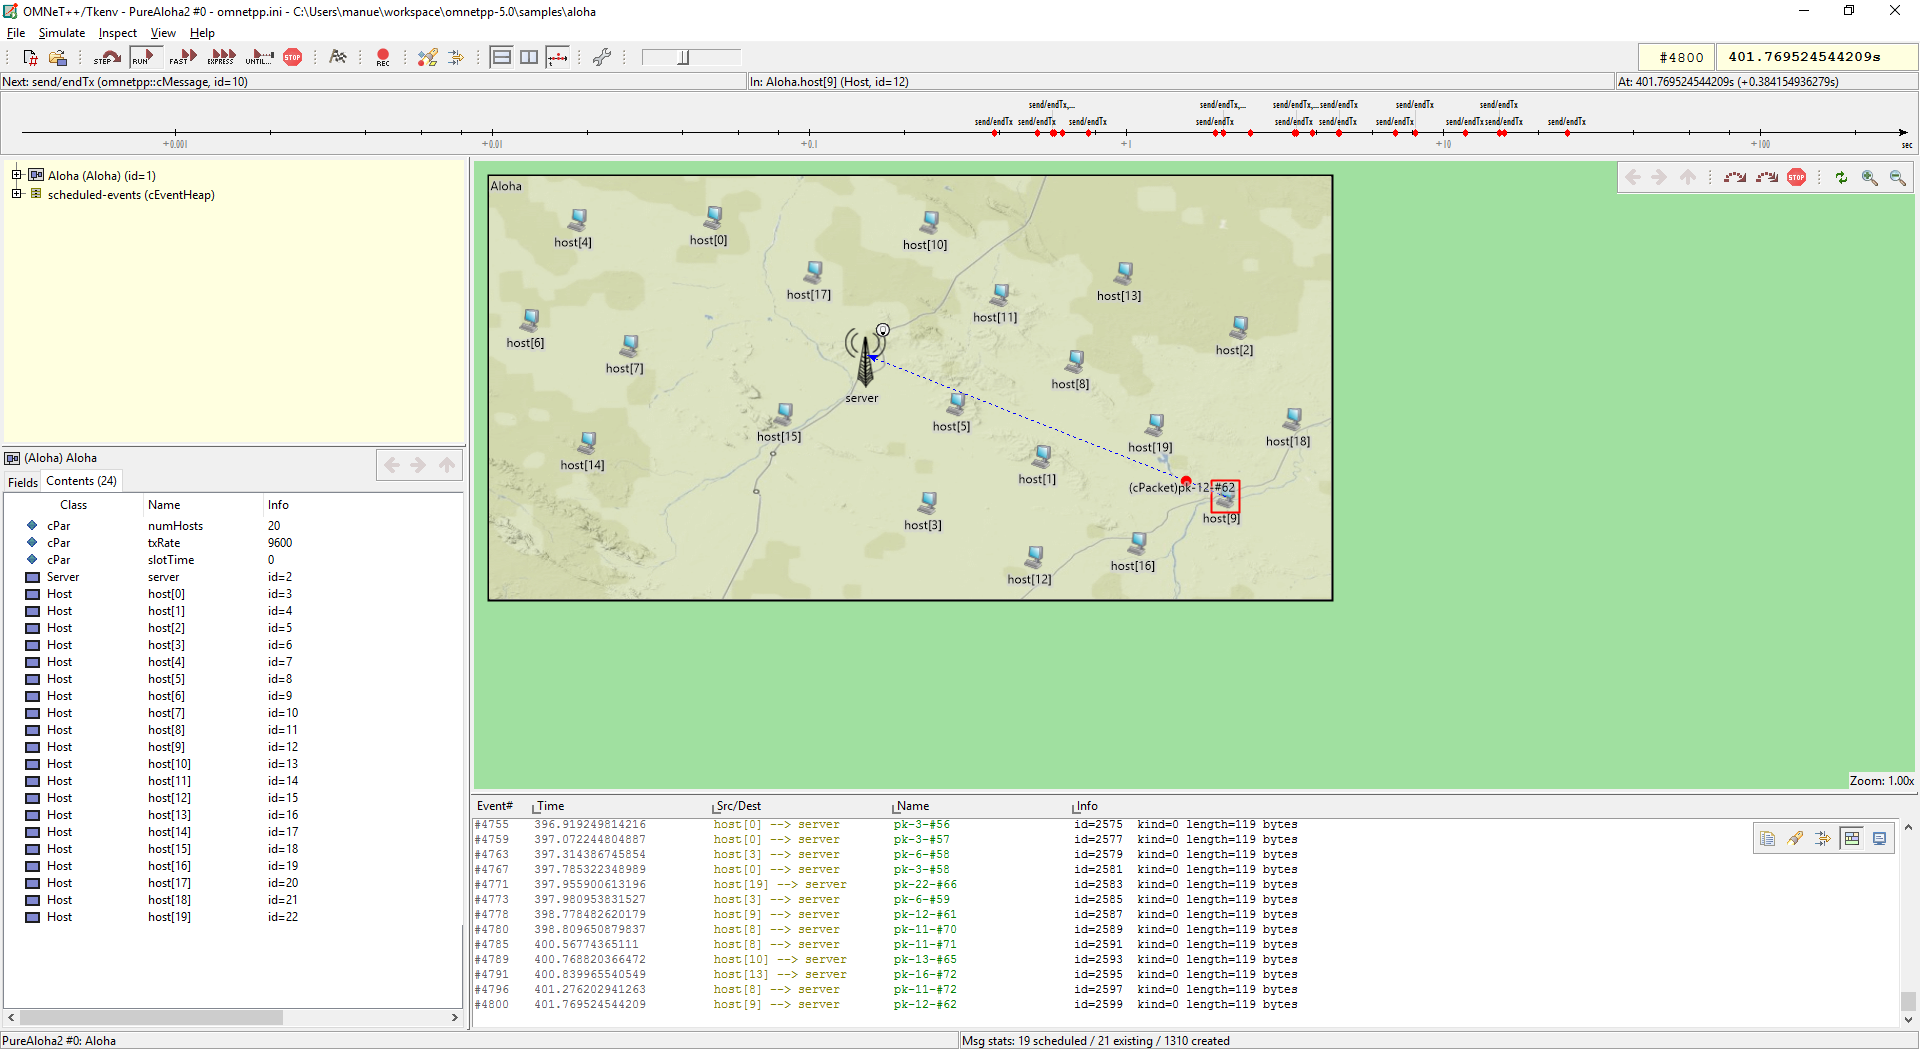
\includegraphics[width=\linewidth]{aloha.png}
  \caption{Entorno gráfico de simulación de OMNeT++}
  \label{fig:omnetgui}
\end{figure}

\subsubsection{SUMO}

SUMO (\emph{Simulation of Urban MObility}) es un simulador de tráfico vehicular de fuente abierta desarrollado originalmente por el Instituto de Sistemas de Transporte del Centro Aeroespacial Alemán (DLR, por sus siglas en alemán -- \emph{Deutsches Zentrum für Luft- und Raumfahrt e.V.}) \cite{sumo}. Es un simulador microscópico, lo cual significa que modela de manera individual y particular cada uno de vehículos presentes en sus simulaciones, a diferencia de simuladores macroscópicos, los cuales modelan el flujo vehicular como un fluído. Esta naturaleza microscópica presenta la ventaja de un mayor realismo en el movimiento de los vehículos en la red de transporte, a cambio de mayores requisitos de capacidad de procesamiento.

Las simulaciones de SUMO se implementan en una serie de archivos XML que describen la red, los vehículos presentes y sus trayectorias y eventual infraestructura no-vial (\emph{polígonos}) presente. Además se debe contar con un archivo \emph{.cfg} que describa los parámetros propios de la simulación (por ejemplo, tiempo de inicio, el largo de cada instante de simulación y el tiempo final).

\begin{figure}[ht]
  \centering
  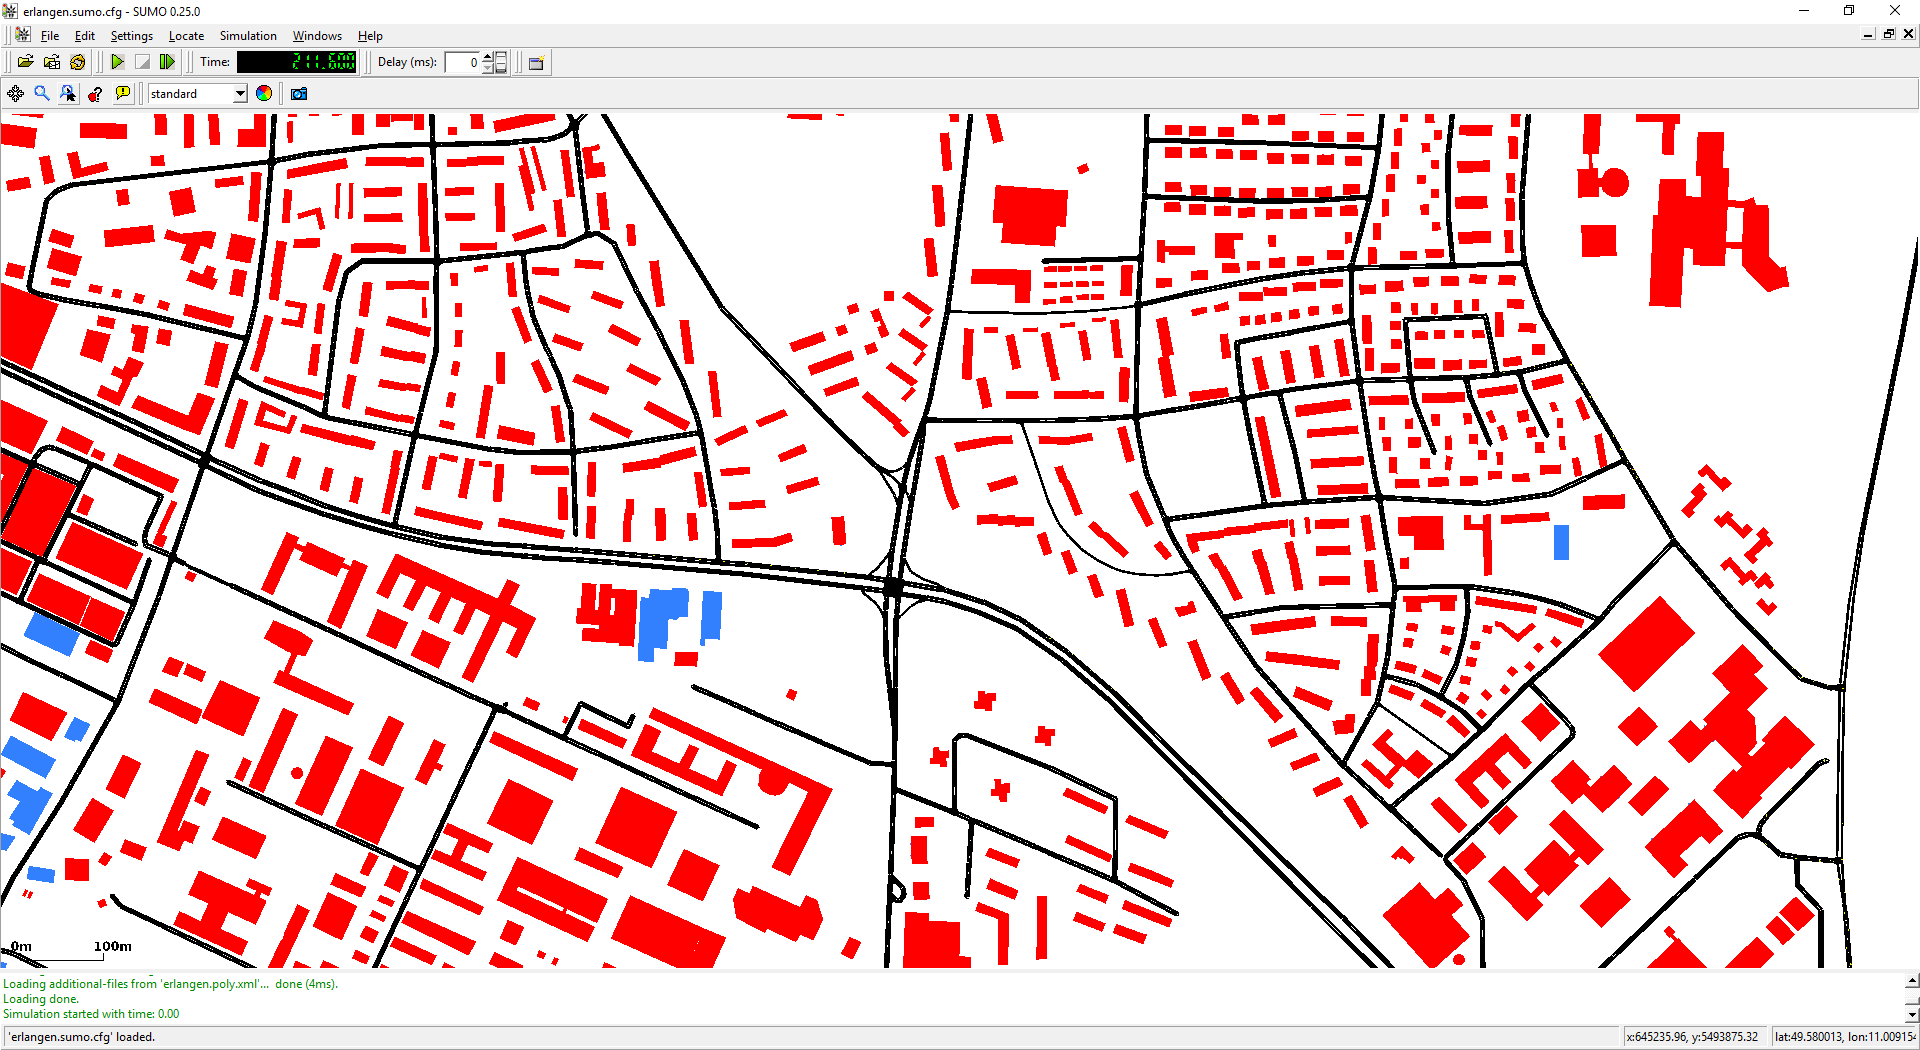
\includegraphics[width=\linewidth]{sumo_demo.png}
  \caption{Simulación de una red en SUMO}
  \label{fig:sumo_demo}
\end{figure}

\subsubsection{VEINS}

\emph{VEhicles In Network Simulation}, \emph{VEINS}, es un \emph{framework} de fuente abierta para la simulación, tanto en su aspecto de comunicaciones como de transporte, de Sistemas de Transporte Inteligente a través de la integración de OMNeT++ con SUMO.

A través de VEINS, estos simuladores se ejecutan en paralelo, comunicándose en tiempo real mediante un \textit{socket} utilizando el protocolo TCP; SUMO proporciona las trazas de movimiento de los elementos en la simulación a la vez que OMNeT++ simula el comportamiento de la red de comunicaciones. Además, mediante este esquema, OMNeT++ también puede modificar directamente el comportamiento del modelo de transporte, por ejemplo alterando la velocidad de un vehículo en respuesta a un mensaje específico obtenido a través de la red de comunicaciones. De esta manera, el \textit{framework} en cuestión permite modelar sistemas complejos y dinámicos, que reflejan de buena manera la realidad, en donde, por ejemplo, un conductor podría reaccionar a información sobre un accidente más adelante en su ruta, alterando su trayectoria para evitar la calle afectada.


\subsection{Situación Previa}\label{section:situacion_previa}

Antes de la llegada del practicante existía poco avance en las tareas propuestas. Si bien la estudiante anterior que había comenzado a trabajar en este tema (Javiera Born, ex-alumna del Departamento de Ciencias de la Computación) ya había construído un escenario simple de SUMO, no se había implementado en VEINS y OMNeT++ todavía, por lo que era una simulación simple y sin inteligencia. De todos modos, dicho escenario sirvió como una excelente base para la primera etapa de la práctica.

\newpage
\section{Trabajo Realizado}

El trabajo realizado tenía como fin último la elaboración de un prototipo de un sistema de alerta temprana para ciclistas en un ITS. El objetivo de este sistema es el de predecir, mediante un modelo de probabilidades bayesianas descrito por Liebner \textit{et al.} en \cite{prediction-paper}, la probabilidad de un giro sorpresivo de un vehículo en un cruce, y notificar esto a ciclistas cercanos a dicho cruce (se asumieron ciclistas y vehículos en el contexto de un ITS, dotados de capacidades de comunicación inalámbrica), con el fin de reducir las colisiones entre automóviles y ciclistas -- y potencialmente salvando vidas.

Este trabajo se dividió en dos partes:

\begin{enumerate}
  \item Estudio y comprensión del software especializado OMNeT++, SUMO y VEINS, y la posterior elaboración de un prototipo simple para ilustrar la factibilidad del proyecto.
  \item Implementación del sistema, utilizando como base el prototipo anterior y utilizando registros de tráfico real.
\end{enumerate}

Cabe destacar que las labores del practicante abarcaron la implementación del modelo vehicular y la integración del modelo predictivo a este. El estudio y la implementación del modelo descrito en \cite{prediction-paper} quedó a cargo de Sebastián Piña M., alumno del DIE y compañero de equipo del practicante.

\subsection{Estudio del software y elaboración de un prototipo inicial simple}

El primer mes de la práctica se enfocó totalmente en el estudio del software especializado, concentrado principalmente en VEINS y la elaboración de modelos de sistemas de transporte inteligentes utilizando el framework. Como un \emph{bonus} adicional, esto significó el aprendizaje de C++ por parte del practicante. Con el fin de realizar un aprendizaje didáctico y aplicado, se implementó además un prototipo simple de un cruce vehicular con carriles para ciclistas, el cual se describe a continuación.

\subsubsection{Prototipo inicial}

El prototipo inicial se construyó en base al trabajo previamente realizado por Javiera Born (descrito en la sección \ref{section:situacion_previa}). Este consistió en una simulación muy simple, compuesta por un vehículo motorizado y una bicicleta, los cuales interactúan en un cruce. Si bien esta simulación presenta un escaso valor práctico y académico, fue de gran ayuda para que el practicante adquiriera las habilidades necesarias para el manejo del software especializado.

\begin{figure}[ht]
  \centering
  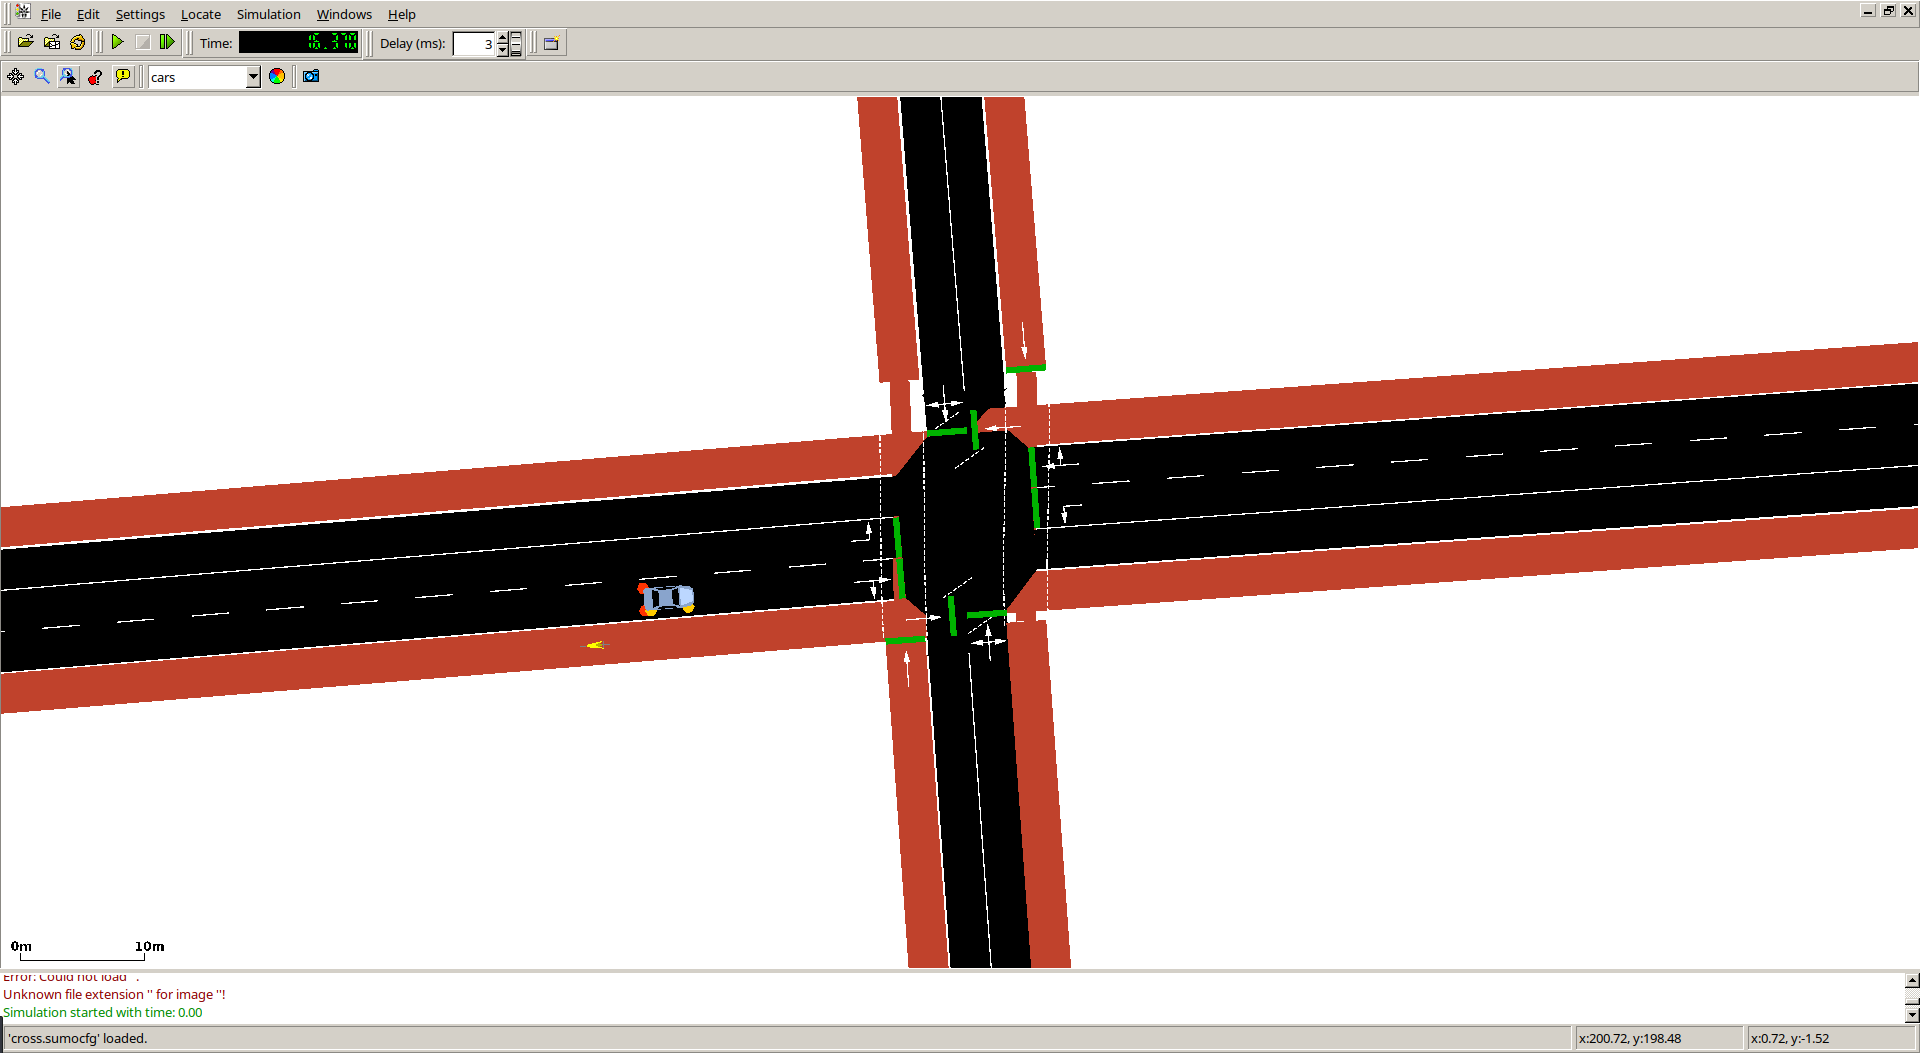
\includegraphics[width=\linewidth]{prototipo_inicial.png}
  \caption{Prototipo inicial en ejecución}
  \label{fig:sumo_prototype}
\end{figure}

\subsubsection{Implementación en SUMO}

El aspecto de transporte de la simulación no presenta grandes cambios respecto a lo desarrollado anteriormente por J. Born -- se reutilzó el cruce vehicular simple compuesto por una vía de tres pistas y otra de dos, ambas con ciclovías a los costados. Se modificaron los flujos vehiculares para que consistieran únicamente en un automóvil y una bicicleta, y para sincronizar su llegada al cruce y poder simular la detención de la bici en reacción a un mensaje de viraje emitido por el automóvil (detalles de la implementación de esto en la sección \ref{section:prot_communication}). Ver figura \ref{fig:sumo_prototype} para una ilustración del modelo en SUMO.

\subsubsection{Implementación en OMNeT++}\label{section:prot_communication}

La lógica de la simulación se implementó en un módulo de OMNeT++ llamado \emph{BikeManeuver}. El comportamiento de ambos vehículos fue implementado en este único módulo; al iniciar la simulación, se verifica (entre otros parámetros) el identificador del vehículo, en base a lo cual se asigna un valor a un \emph{flag} que determina el comportamiento del módulo en el resto de la simulación.

Cada vehículo fue modelado como una máquina de estados finita, los cuales cambian de estado en respuesta a estímulos exteriores y/o interiores (la figura \ref{diag:states} ilustra estos diagramas de estado). A continuación se detalla el comportamiento de ambos, y el código \ref{lst:simple_car_fsm} expone un extracto del código del módulo.

\begin{description}[leftmargin=!,labelwidth=\widthof{\bfseries Automóvil}]
    \item [Bicicleta]  El comportamiento de este vehículo es simple. El módulo espera hasta recibir un mensaje de advertencia desde el automóvil; al recibirlo, verifica la distancia actual de la bicicleta al cruce. De ser esta menor a una distancia $D$ establecida, la bicicleta se detiene hasta recibir un segundo mensaje del automóvil, el cual confirma que este último ha finalizado su giro. Finalmente, la bicicleta resume su trayectoria hasta terminar la simulación.
    \item [Automóvil]  El automóvil tiene un comportamiento ligeramente más complicado, ya que debe constantmente estar monitoreando su distancia al cruce para determinar cuándo emitir los mensajes que espera la bicicleta. Para esto, al principio de la simulación se programa un ``automensaje'' (\emph{selfbeacon} en inglés) a ser enviado por el módulo a si mismo en el siguiente instante de simulación ($0.1$s más tarde). Al recibir dicho mensaje, se programa un nuevo \emph{selfbeacon} y se verifica si la distancia del vehículo al cruce es menor o igual a la distancia $D$ previamente mencionada. De ser así, se emite el primer mensaje de advertencia, y se cambia el estado a ``girando'', hasta detectar (mediante la misma técnica anterior de mediciones periódicas) que se encuentra nuevamente fuera del cruce (distancia $\geq D$), momento que se emite el segundo y último mensaje y se vuelve a la operación normal.
\end{description}

Cabe notar que la técnica de uso de \emph{selfbeacons} para realizar operaciones periódicas en OMNeT++ es altamente común, y fue uno de los principales aprendizajes de esta estapa del trabajo de práctica \cite{selfmessage}.


\begin{figure}
    \centering
    \subfloat[Bicicleta]{
        \begin{tikzpicture}[scale=0.17, align=center]
            \tikzstyle{every node}+=[inner sep=0pt]
            \draw [black] (13,-12.8) circle (3);
            \draw (13,-12.8) node {IDLE};
            \draw [black] (35.7,-12.8) circle (3);
            \draw (35.7,-12.8) node {GO};
            \draw [black] (35.7,-38.2) circle (3);
            \draw (35.7,-38.2) node {CHECK};
            \draw [black] (62.6,-25.8) circle (3);
            \draw (62.6,-25.8) node {STOP};
            \draw [black] (6.7,-12.8) -- (10,-12.8);
            \fill [black] (10,-12.8) -- (9.2,-12.3) -- (9.2,-13.3);
            \draw [black] (16,-12.8) -- (32.7,-12.8);
            \fill [black] (32.7,-12.8) -- (31.9,-12.3) -- (31.9,-13.3);
            \draw (24.35,-13.3) node [below] {SIM START};
            \draw [black] (37.012,-15.496) arc (22.64734:-22.64734:25.981);
            \fill [black] (37.01,-35.5) -- (37.78,-34.96) -- (36.86,-34.57);
            \draw (39.52,-25.5) node [right] {MSG:\\WARNING};
            \draw [black] (34.393,-35.501) arc (-157.45725:-202.54275:26.088);
            \fill [black] (34.39,-15.5) -- (33.62,-16.05) -- (34.55,-16.43);
            \draw (31.9,-25.5) node [left] {d $\geq$ D};
            \draw [black] (60.563,-28.001) arc (-45.23709:-85.26667:35.174);
            \fill [black] (60.56,-28) -- (59.64,-28.21) -- (60.35,-28.92);
            \draw (53.86,-35.5) node [below] {d $<$ D};
            \draw [black] (38.693,-12.624) arc (90.29696:38.11674:28.013);
            \fill [black] (38.69,-12.62) -- (39.5,-13.12) -- (39.49,-12.12);
            \draw (57.84,-14.87) node [above] {MSG: DONE};
        \end{tikzpicture}
    }
    \par\medskip
    \subfloat[Automóvil]{
        \begin{tikzpicture}[scale=0.17, align=center]
            \tikzstyle{every node}+=[inner sep=0pt]
            \draw [black] (14.9,-7.3) circle (3);
            \draw (14.9,-7.3) node {INIT};
            \draw [black] (34.9,-7.3) circle (3);
            \draw (34.9,-7.3) node {IDLE};
            \draw [black] (64.7,-7.3) circle (3);
            \draw (64.7,-7.3) node {CHECK};
            \draw [black] (64.7,-22.1) circle (3);
            \draw (64.7,-22.1) node {BROADCAST\\WARNING};
            \draw [black] (64.7,-37.3) circle (3);
            \draw (64.7,-37.3) node {TURN};
            \draw [black] (34.9,-38) circle (3);
            \draw (34.9,-38) node {CHECK};
            \draw [black] (34.9,-22.1) circle (3);
            \draw (34.9,-22.1) node {BROADCAST\\DONE};
            \draw [black] (17.9,-7.3) -- (31.9,-7.3);
            \fill [black] (31.9,-7.3) -- (31.1,-6.8) -- (31.1,-7.8);
            \draw (24.9,-7.8) node [below] {SIM START};
            \draw [black] (37.821,-6.618) arc (101.69073:78.30927:59.118);
            \fill [black] (61.78,-6.62) -- (61.1,-5.97) -- (60.89,-6.95);
            \draw (49.8,-4.89) node [above] {SELFMESSAGE};
            \draw [black] (61.825,-8.156) arc (-75.23743:-104.76257:47.192);
            \fill [black] (37.77,-8.16) -- (38.42,-8.84) -- (38.68,-7.88);
            \draw (49.8,-10.21) node [below] {d $>$ D};
            \draw [black] (64.7,-10.3) -- (64.7,-19.1);
            \fill [black] (64.7,-19.1) -- (65.2,-18.3) -- (64.2,-18.3);
            \draw (65.2,-14.7) node [right] {d $\leq$ D};
            \draw [black] (64.7,-25.1) -- (64.7,-34.3);
            \fill [black] (64.7,-34.3) -- (65.2,-33.5) -- (64.2,-33.5);
            \draw [black] (61.922,-38.43) arc (-70.12101:-107.18774:38.068);
            \fill [black] (37.73,-39) -- (38.34,-39.71) -- (38.64,-38.76);
            \draw (49.93,-41.31) node [below] {SELFMESSAGE};
            \draw [black] (37.655,-36.815) arc (110.90833:71.78292:36.203);
            \fill [black] (61.89,-36.25) -- (61.29,-35.52) -- (60.98,-36.47);
            \draw (49.69,-33.86) node [above] {d $<$ D};
            \draw [black] (34.9,-35) -- (34.9,-25.1);
            \fill [black] (34.9,-25.1) -- (34.4,-25.9) -- (35.4,-25.9);
            \draw (35.4,-30.05) node [right] {d $\geq$ D};
            \draw [black] (8.7,-7.3) -- (11.9,-7.3);
            \fill [black] (11.9,-7.3) -- (11.1,-6.8) -- (11.1,-7.8);
            \draw [black] (34.9,-19.1) -- (34.9,-10.3);
            \fill [black] (34.9,-10.3) -- (34.4,-11.1) -- (35.4,-11.1);
        \end{tikzpicture}
    }
    \caption[Diagramas de estado: Bicicleta y Automóvil]{Diagramas de estado de bicicleta y automóvil. Notar que se representan también estados transitorios, para los cuales no se estimó necesario crear un estado ``real'' en la implementación.}
    \label{diag:states}
\end{figure}

\newpage
\subsection{Modelación del sistema de alarma temprana}

Como se mencionó anteriormente, la segunda etapa del trabajo contemplaba la implementación de un sistema de alarma temprana para ciclistas en cruces no regulados, basado en el trabajo de Liebner \emph{et al.}, descrito en \cite{prediction-paper}. En esta publicación, los autores detallan un modelo predictivo del comportamiento de vehículos en intersecciones urbanas, basado en la teoría de probabilidades bayesianas.

En términos muy simplificados, el modelo predictivo se basa en la categorización de los conductores en base a su comportamiento vial (aceleración promedio, velocidad máxima, etc.), para luego contrastar su comportamiento al acercarse a un cruce. En base a esta comparación, se calcula la probabilidad del giro.

\subsubsection{Implementación en SUMO}

Se optó por utilizar un escenario de SUMO con trazas vehiculares reales; es decir, un registro real del tráfico en una ciudad. De esta manera se asegura un alto grado de realismo del comportamiento de los vehículos en la simulación, lo cual es un requisito fundamental para la validación de los resultados obtenidos.

El escenario \emph{TAPAS Cologne} \cite{tapascologne} fue el escogido para este fin, dada la calidad y la cantidad de datos que incluye. Este escenario describe el flujo vehicular en la ciudad de Cologne, en Alemania, durante un día completo, tanto para vehículos particulares como para el transporte público, en un mapa que abarca la ciudad en su totalidad. Por conveniencia, incluye dos sub-escenarios distintos, uno que describe completamente 24 horas de tráfico vehicular, y otro que contiene información de sólo dos horas (entre 6:00 y 8:00 a.m.). Fue este último el utilizado para el desarrollo del sistema de alarma temprana, el cual además se adaptó a la naturaleza del sistema a modelar.

Dado que el sistema contempla el monitoreo de una intersección, se decidió escoger un cruce apropiado y sólo incluir las trazas de movimiento vehicular que lo incluyeran en su trayectoria. La elección del cruce se hizo de manera manual, ya que no requiere condiciones estrictas, siguiendo los siguientes pasos:

\begin{enumerate}
	\item Se seleccionó primero un grupo semi-arbritrario de intersecciones a considerar, sin semáforos y de cantidad de pistas reducidas. La primera condición es de carácter funcional -- la existencia de un semáforo se asume que elimina la necesidad de un sistema predictivo de giros sorpresivos. La segunda es de carácter más práctico; una intersección con muchas pistas agrega complejidad innecesaria a un modela en tan temprana etapa de desarrollo.
	\item En segundo lugar, se analizaron los flujos vehiculares de cada uno de los cruces seleccionados, descartando aquellos que presentaran nula o poca presencia vehicular a lo largo de la simulación.
	\item Finalmente se hizo la elección final, en base a la simplicidad total del cruce.
\end{enumerate}

La intersección finalmente seleccionada para la simulación fue el cruce $55063174$, compuesto por la intersección de los \emph{arcos} (calles) $132530717$, $132530803$, $7651840$ y $132530803$, caracterizada por ser un cruce entre dos calles de una pista cada una, lo cual tiene la ventaja de que limita los virajes a considerar a únicamente dos direcciones distintas. Este cruce fue modificado levemente además para incluir ciclovías al costado de ambas calles, ya que el escenario \emph{TAPAS Cologne} no incluye registros de este medio de transporte.

Por otro lado, las trazas vehiculares incluídas en el escenario también debieron ser alteradas y filtradas. Dichas trazas están descritas en archivos XML (ver código \ref{sumo:routes}), compuestos por dos tipos esenciales de elementos; vehículos y rutas. Una ruta consiste en una serie de identificadores de \emph{arcos} que forman un recorrido desde una posición inicial $A$ hasta un destino $B$. Estas se asocian luego a vehículos, describiendo de esta manera el movimiento de éstos últimos por la red vehicular. Puesto que, para los fines de la simulación en cuestión, sólo interesaban aquellos vehículos que se desplazaran por la intersección seleccionada anteriormente, se optó por filtrar el archivo de rutas, eliminando todos aquellos vehículos no relevantes para el trabajo. Esto se efectuó utilizando un script escrito en Python (ver código \ref{sumo:py_filter}), y redujo el tamaño del archivo de rutas de aproximadamente 200 MB a sólo 1.5 MB, lo cual aceleró de manera considerable el tiempo de carga y de inicio del escenario en SUMO.

Finalmente, se optó además por no incluir información de la infraestructura presente en la ciudad en la simulación, ya que 1. agregaba considerable \emph{overhead} a la carga y ejecución del escenario y 2. el rango de comunicación inalámbrica a efectuar es lo suficientemente acotado como para poder desestimar el impacto posible de edificios y estructuras en las cercanías del cruce (por lo menos en las etapas tempranas de desarrollo).

\begin{figure}
	\centering
	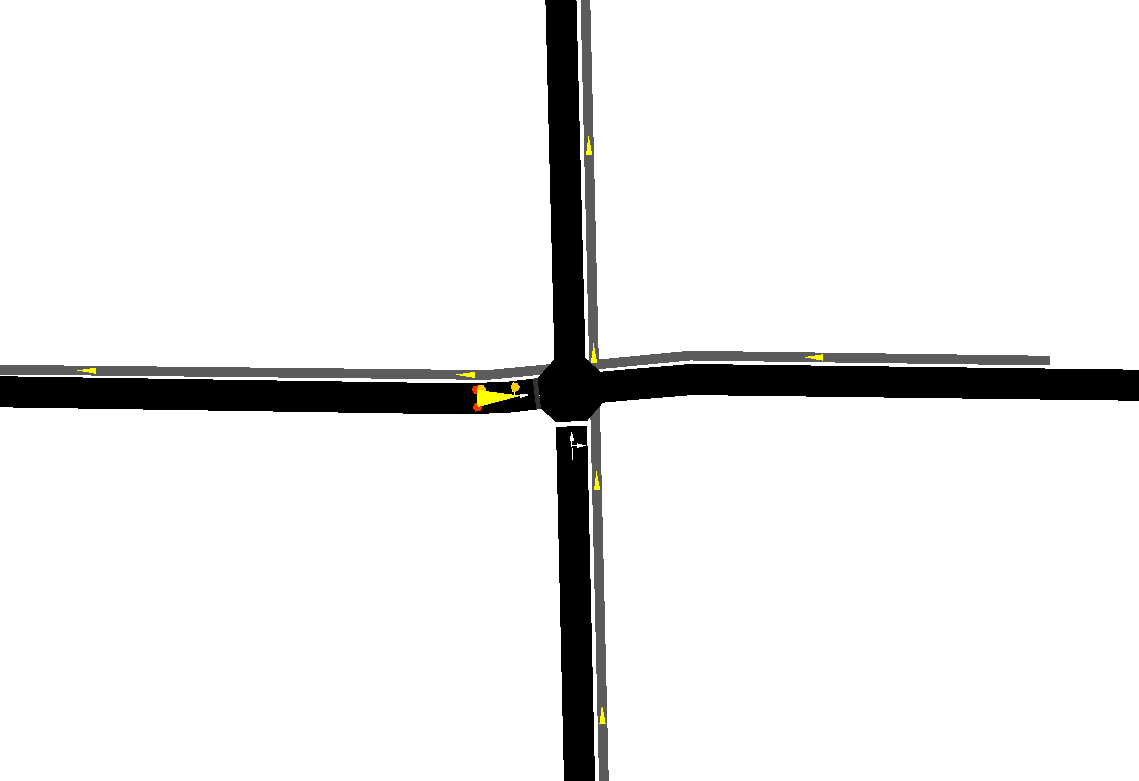
\includegraphics[width=\linewidth]{junction.png}
	\caption[Cruce $55063174$]{\emph{Zoom} del cruce $55063174$, escogido para la implementación del sistema de alarma temprana.}
	\label{sumo:junction}
\end{figure}

\noindent\begin{minipage}{\linewidth}
\begin{lstlisting}[style=m_xml, label={sumo:routes}, caption={Extracto de trazas vehiculares del escenario TAPAS Cologne. Cada vehículo tiene asociada una ruta, la cual describe el camino que recorre este desde su origen hasta su destino.}]
<vehicle id="37937_37937_358_0" type="pkw" depart="21600.00">
    <route edges="328974180 133852448-AddedOnRampEdge 133852448 7854060 ..."/>
</vehicle>
<vehicle id="38648_38648_359_0" type="pkw" depart="21600.00">
    <route edges="51793889 -155592914#2 -155592914#1 155592907#2 155592972 ..."/>
</vehicle>
<vehicle id="38750_38750_359_0" type="pkw" depart="21600.00">
    <route edges="8437608#3 -8437608#6 -8437608#2 -189913664#3 -209682829#1 ..."/>
</vehicle>
<vehicle id="41314_41314_361_0" type="pkw" depart="21600.00">
    <route edges="25326879#0 24609080#3 118427328#0 118427328#2 118427328#3 ..."/>
</vehicle>
<vehicle id="41690_41690_361_0" type="pkw" depart="21600.00">
    <route edges="29337995#1 29337995#3 29337995#5 29337995#7 9250113#2 ..."/>
</vehicle>
<vehicle id="43455_43455_362_0" type="pkw" depart="21600.00">
    <route edges="340575954#3 99714977#3 99714977#4 196122462#0 27892605#0 ..."/>
</vehicle>
\end{lstlisting}
\end{minipage}

\noindent\begin{minipage}{\linewidth}
\begin{lstlisting}[style=mPython, caption={Código de extracción de vehículos relevantes.}, label={sumo:py_filter}]
import xmltodict

EDGES = ['132530717#0', '132530803#1', '7651840#0', '132530803#0']

with open('cologne6to8.rou.xml', 'r') as infile, \
        open('cologne6to8.filtered.rou.xml', 'w') as outfile:
    orig_xml = xmltodict.parse(infile.read())
    vehicles = orig_xml['routes']['vehicle']
    relevant_vehicles = []

    for v in vehicles:
        edges = v['route']['@edges'].split(' ')
        for e in EDGES:
            if e in edges and v not in relevant_vehicles:
                relevant_vehicles.append(v)

    orig_xml['routes']['vehicle'] = relevant_vehicles
    outfile.write(xmltodict.unparse(orig_xml, pretty=True))

    print(
        '''
Done. Filtered on edges: {e}.
Final results: {i} cars match the desired edges.
        '''.format(e=EDGES, i=len(relevant_vehicles))
    )
\end{lstlisting}
\end{minipage}

\subsubsection{Implementación en OMNeT++}

El escenario contempla tres tipos de entidades diferentes que interactúan en el cruce:

\begin{description}[leftmargin=!,labelwidth=\widthof{\bfseries Automóviles}]
	\item [RSU]	La unidad de infraestructura inteligente, \emph{RSU} (por sus siglas en inglés, \emph{RoadSide Unit}), no ``existe'' en el escenario físico, sino que es creada y trasladada al centro de la intersección por OMNeT++ al iniciarse la simulación. La RSU tiene como labor la interpretación del estado del sistema en cada instante de tiempo; recibe datos desde los vehículos presentes y es la entidad que detecta un viraje sorpresivo y emite la advertencia correspondiente.

	La funcionalidad de esta fue separada en múltiples archivos. En primer lugar, la clase \emph{BikeWarningRSU} extiende un módulo básico de OMNeT++ equipado con interfaces inalámbricas. En este se implementó la comunicación del módulo con el resto de las entidades de la simulación; en específico, la RSU recibe \emph{beacons} periódicos desde los automóviles, los cuales contienen información posicional de los vehículos, como su velocidad y posición. Esta información luego es proporcionada como parámetros al algoritmo de decisión -- si la determinación de éste último es positiva, la RSU emite una advertencia en modo \emph{broadcast} a todos los vehículos presentes en la simulación. En caso contrario se descarta el resultado.

	El algoritmo de decisión en sí fue implementado en Python por S. Piña, y fue integrado a la simulación mediante la clase de C++ \emph{DecisionAlgorithm}, utilizando código Python embebido (ver código \ref{lst:embedded_python}). Esta clase inicializa la interfaz con Python, y presenta funciones de conveniencia para interactuar directamente con la implementación del algoritmo desde C++.

	\item [Automóviles]	Los automóviles en esta simulación carecen de inteligencia, en el sentido que no cuentan con inteligencia propia más allá de la lógica de recolección de información que luego es enviada a la RSU. Su funcionalidad se implementó en el módulo de OMNeT++ \emph{BikeWarningApplication}.

	Esta clase utiliza el mismo método de \emph{selfbeacons} detallado en la etapa anterior de la práctica para periódicamente medir los parámetros físicos del vehículo (posición, velocidad y calle actual) y enviarlos a la RSU (ver código \ref{lst:send_json}). Para este fin se utilizó el formato de mensaje por defecto del protocolo \emph{WAVE} (\emph{Wireless Access for Vehicular Environments}, una variante del estándar IEEE802.11 para comunicaciones en contextos de sistemas de transporte inteligentes \cite{80211wave}). La implementación de este mensaje en OMNeT++ sólo cuenta con un campo de texto para el \emph{payload}, por lo cual la información requerida debió codificarse en \emph{JSON} antes de ser enviada. El código \ref{lst:send_json} ilustra el método encargado de la recolección y envío de datos en el módulo.
	\item [Bicicletas]	Finalmente, las bicicletas también se implementaron en \emph{BikeManeuver}, sin embargo su comportamiento es aún más simple que el de los automóviles. Simplemente monitorean de manera pasiva las emisiones del RSU, y al recibir una advertencia se detienen por un periodo de tiempo predeterminado antes de seguir su trayectoria normal. Se decidió optar por esta simplicidad para priorizar primero la validación del funcionamiento fundamental de la teoría antes de implementar un modelo más complejo.
\end{description}

\noindent\begin{minipage}{\linewidth}
\begin{lstlisting}[style=CPP, caption={Código encargado de la medición periódica y envío de datos a la RSU en \emph{BikeWarningApplication}.}, label={lst:send_json}]
void BikeWarningApplication::carHandleSelfMsg(cMessage *msg)
{
    switch (msg->getKind()) {
            case SEND_BEACON_EVT: {
                //std::cout << "Sending beacon: ";
                WaveShortMessage* wsm = prepareWSM("beacon", beaconLengthBits,
													type_CCH, beaconPriority,
													-1, -1);

				// get current position, speed, lane and id
                Coord pos = mobility->getCurrentPosition();
                double speed = mobility->getSpeed();
                std::string id = mobility->getExternalId();
                std::string lane_id = traciVehicle->getLaneId();

				// encode into JSON for easy packing into WAVE short message.
                json data_j = {
                        {"id", id},
                        {"vel", speed},
                        {"pos_x", pos.x},
                        {"pos_y", pos.y},
                        {"lane_id", lane_id}
                };

                std::string jdata = data_j.dump();
                //std::cout << jdata << std::endl;

				// load payload into message and send it
                wsm->setWsmData(jdata.c_str());
                sendWSM(wsm);
                scheduleAt(simTime() + par("beaconInterval").doubleValue(), sendBeaconEvt);
                break;
            }
            default: {
                if (msg)
                    DBG << "APP: Error: Got Self Message of unknown kind! Name: " << msg->getName() << endl;
                break;
            }
        }
}
\end{lstlisting}
\end{minipage}


\newpage
\section{Conclusiones}

En términos de los objetivos planteados al inicio de la práctica, se evalúa de manera positiva el trabajo realizado por el practicante. Se lograron los principales objetivos de aprendizaje de software especializado y de teoría de sistemas de transportes inteligentes.

Se lograron buenos resultados parciales, los cuales fueron presentados en el \emph{Taller de Inteligencia Urbana} en Santa Cruz, Región de O'Higgins, en Noviembre del 2016 por S. Piña. Además, se presentó un borrador inicial del trabajo al profesor Falko Dressler (uno de los creadores de VEINS, y un reconocido investigador en el área de Sistemas de Transporte Inteligente) en su visita a Chile a principios de Agosto, recibiendo un alto grado de optimismo respecto a la investigación por parte del académico.

El trabajo tuvo un profundo impacto y gran interés en el practicante, específicamente en el tema de simuladores para ITS. Actualmente, este interés se ha visto concretado en un trabajo de memoria a desarrollarse durante el presente semestre.

Desafortunadamente, a pesar del trabajo realizado, la simulación no fue del todo fructuosa y hasta el día de hoy su desarrollo se encuentra congelado hasta nuevo aviso. El principal problema surge de que la teoría predictiva está basada en el estudio del comportamiento de los vehículos dada la existencia de otro vehículo en la pista, frente al primero, y la adaptación de este modelo a uno basado únicamente en los datos individuales de cada vehículo presentó problemas inesperados.

\newpage
\begin{thebibliography}{5}
    \bibitem{TICS} \emph{Tecnologías de la Información y Comunicaciones} - \url{https://es.wikipedia.org/wiki/Tecnolog%C3%ADas_de_la_informaci%C3%B3n_y_la_comunicaci%C3%B3n}

    \bibitem{scespedes} \emph{Sandra Céspedes U.} - \url{http://www.cec.uchile.cl/~scespedes/}

    \bibitem{DIE} \emph{Departamento de Ingeniería Eléctrica} - \url{http://die.cl/}

    \bibitem{eudirective}
  		\hbadness=1000 Directive 2010/40/EU of the European Parliament and of the Council
  		\textit{on the framework for the deployment of Intelligent Transport Systems in the field of road transport and for interfaces with other modes of transport},
  		2010 O.J. L 207/1

    \bibitem{usdot}
  		\hbadness=1000 U.S. Department of Transportation
  		\textit{Office of the Assistant Secretary for Research and Technology (OST-R)}
  		\\\url{http://www.itsoverview.its.dot.gov/} (\textit{04/2017})

    \bibitem{80211dailey}
  		\hbadness=1000 D. J. Dailey, K. McFarland and J. L. Garrison
  		\textit{Experimental study of 802.11 based networking for vehicular management and safety},
  		Intelligent Vehicles Symposium (IV), 2010 IEEE, San Diego, CA, 2010, pp. 1209-1213.
  		\\doi: 10.1109/IVS.2010.5547955


  	\bibitem{80215vanet}
  		\hbadness=1000 W. Xiong; X. Hu; T. Jiang.
  		\textit{Measurement and Characterization of Link Quality for IEEE 802.15.4-compliant Wireless Sensor Networks in Vehicular Communications},
  		IEEE Transactions on Industrial Informatics , vol.PP, no.99, pp.1-1
  		\\doi: 10.1109/TII.2015.2499121

  	\bibitem{80211wave}
  		\hbadness=1000 D. Jiang and L. Delgrossi.
  		\textit{IEEE 802.11p: Towards an International Standard for Wireless Access in Vehicular Environments}, Vehicular Technology Conference, 2008. VTC Spring 2008. IEEE, Singapore, 2008, pp. 2036-2040.
  		\\doi: 10.1109/VETECS.2008.458

	\bibitem{v2vlte}
		\hbadness=1000 S. Kato, M. Hiltunen, K. Joshi and R. Schlichting
		\textit{Enabling vehicular safety applications over LTE networks},
		2013 International Conference on Connected Vehicles and Expo (ICCVE), Las Vegas, NV, 2013, pp. 747-752.
		\\doi: 10.1109/ICCVE.2013.6799889

    \bibitem{omnet}
  		\hbadness=1000 OMNeT++ Discrete Event Simulator.
  		\textit{An extensible, modular, component-based C++ simulation library and framework, primarily for building network simulators}.
  		\\\url{https://OMNeTpp.org/} (\textit{04/2017})

    \bibitem{sumo}
  		\hbadness=1000 SUMO – Simulation of Urban MObility.
  		\textit{A free and open traffic simulation suite which is available since 2001.}
  		\\\url{http://sumo.dlr.de} (\textit{4/2017})

    \bibitem{prediction-paper}
      \hbadness=1000 M. Liebner, F. Klanner, M. Baumann, C. Ruhhammer and C. Stiller.
      \textit{Velocity-Based Driver Intent Inference at Urban Intersections in the Presence of Preceding Vehicles},
      IEEE Intelligent Transportation Systems Magazine, vol. 5, no. 2, pp. 10-21, Summer 2013.
      \\doi: 10.1109/MITS.2013.2246291

	\bibitem{selfmessage}
	  \hbadness=1000 OMNeT++ Simulation Manual
	  \textit{4.7.1 Self-Messages}
	  \\\url{https://omnetpp.org/doc/omnetpp/manual/#sec:simple-modules:self-messages} (\textit{4/2017})

	\bibitem{tapascologne}
	  \hbadness=1000 TAPAS Cologne
	  \textit{Scenario describing the traffic in the city of Cologne, Germany, during a whole day.}
	  \\\url{http://sumo.dlr.de/wiki/Data/Scenarios/TAPASCologne} (04/2017)

\end{thebibliography}
\newpage
\section{Anexos}

\begin{lstlisting}[style=CPP, label={lst:simple_car_fsm}, caption={Extracto del código encargado del comportamiento del automóvil.}]
FSM_Switch(carFSM)
{
case FSM_Exit(CAR_INIT):
{
	// init simulation: go to car idle state and schedule selfbeacon for
	// periodic checks of distance to junction
    FSM_Goto(carFSM, CAR_IDLE);
    scheduleAt(simTime() + ping_interval, selfbeacon);
    break;
}
case FSM_Exit(CAR_IDLE):
{
    // got a selfbeacon?
    if (msg == selfbeacon)
    {
		// "transitory" state: check distance to crossing.
		// if we are too far away then do nothing apart from scheduling another
		// selfbeacon, otherwise send warning and change state
        if (traci->getDistance(
                traci->junction("cluster_0__0_0__2_0__4_0__6").getPosition(),
                mobility->getCurrentPosition(), false) > 30)
        {
			// too far away, schedule next check
            scheduleAt(simTime() + ping_interval, selfbeacon);
            break;
        }

		// close to the crossing, send warning and start turn
        t_channel channel = dataOnSch ? type_SCH : type_CCH;
        turnmsg = prepareWSM("data", dataLengthBits, channel, dataPriority, -1, 2);
        turnmsg->setWsmData(warning);
        sendWSM(turnmsg);
        scheduleAt(simTime() + ping_interval, selfbeacon);
        FSM_Goto(carFSM, CAR_TURNING);
    }
    break;
}
case FSM_Exit(CAR_TURNING):
{
    // got selfbeacon?
    if (msg == selfbeacon)
	{
		// "transitory" state: check distance to crossing.
		// are we still turning? then do nothing apart from scheduling selfbeacon
		// otherwise, broadcast and return to normal operation
        if (traci->getDistance(
                traci->junction("cluster_0__0_0__2_0__4_0__6").getPosition(),
                mobility->getCurrentPosition(), false) < 30)
        {
			// still turning, do nothing and schedule next check
            scheduleAt(simTime() + ping_interval, selfbeacon);
            break;
        }

		// donde turning, let the bike know!
        t_channel channel = dataOnSch ? type_SCH : type_CCH;
        turnmsg = prepareWSM("data", dataLengthBits, channel, dataPriority, -1, 2);
        turnmsg->setWsmData(warning);
        sendWSM(turnmsg);
        scheduleAt(simTime() + ping_interval, selfbeacon);
        FSM_Goto(carFSM, CAR_IDLE);
    }
    break;
}
}
\end{lstlisting}

\begin{lstlisting}[style=CPP, caption={Llamado a código Python externo desde C++ en el módulo \emph{DecisionAlgorithm}}, label={lst:embedded_python}]
DecisionAlgorithm::DecisionAlgorithm() {
    Py_Initialize();
    PyRun_SimpleString( "import os, sys, random, traceback\n"
                        "sys.path.append(os.getcwd())\n");
    pName = PyUnicode_DecodeFSDefault(DECISION_ALGO_SCRIPT);
    pModule = PyImport_Import(pName);
    if(pModule == NULL)
    {
        std::cout << "Null pModule" << std::endl;
        throw -1;
    }
    pFunc = PyObject_GetAttrString(pModule, DECISION_ALGO_FUNC);
    pAddEntry = PyObject_GetAttrString(pModule, DECISION_ALGO_ADDENTRYLANE);
    pAddExit = PyObject_GetAttrString(pModule, DECISION_ALGO_ADDEXITLANE);

    if(!(pFunc && PyCallable_Check(pFunc)))
    {
        std::cout << "Null Decision Function" << std::endl;
        throw -1;
    }
    else if(!(pAddEntry && PyCallable_Check(pAddEntry)))
    {
        std::cout << "Null Entry Lane Function" << std::endl;
        throw -1;
    }
    else if(!(pAddExit && PyCallable_Check(pAddExit)))
    {
        std::cout << "Null Exit Lane Function" << std::endl;
        throw -1;
    }

}

double DecisionAlgorithm::checkTurn(double velocity, double pos_x, double pos_y, std::string car_id, std::string lane_id)
{

    pArgs = PyTuple_New(5);
    PyTuple_SetItem(pArgs, 0, PyFloat_FromDouble(velocity));
    PyTuple_SetItem(pArgs, 1, PyFloat_FromDouble(pos_x));
    PyTuple_SetItem(pArgs, 2, PyFloat_FromDouble(pos_y));
    PyTuple_SetItem(pArgs, 3, PyByteArray_FromStringAndSize(car_id.c_str(), car_id.length()));
    PyTuple_SetItem(pArgs, 4, PyByteArray_FromStringAndSize(lane_id.c_str(), lane_id.length()));


    PyObject* result = PyObject_CallObject(pFunc, pArgs);
    if(result == NULL)
    {
        std::cerr << "null return, something went wrong" << std::endl;
        throw -1;
    }

    //long final = PyLong_AsLong(result);
    double final = PyFloat_AsDouble(result);
    Py_DECREF(pArgs);

    return final;// == final;
}
\end{lstlisting}


% ============= FIN DE DOCUMENTO ==============
\end{document}
